Correlacionar la mirada del conductor en el espacio resulta de gran interés, ya que permite desarrollar herramientas que integren nuevas variables atencionales en los algoritmos de toma de decisiones, otorgándoles un mayor nivel de naturalismo. Sin embargo, se encuentran pocos estudios donde se desarrolle una fusión de la mirada del conductor con los elementos del entorno de forma automática. Algunos programas sofisticados están trabajando en soluciones basadas en inteligencia artificial, como es el ejemplo de SmartEye, que permite la identificación de la atención del usuario a la vez que la determinación de la naturaleza del objeto mirado. Pero la realidad es que muchos ensayos de seguimiento visual se siguen procesando de manera manual, realizando codificaciones en las imágenes o vídeos sobre el tipo de evento observado, cuya tarea puede ser bastante tediosa e inexacta en función de la duración del ensayo.

La integración de la mirada del conductor hacia el exterior del vehículo requiere de un paso intermedio que permita referenciar todos los sistemas en un origen de coordenadas común. La clave de esta cuestión reside en la determinación del movimiento de la cabeza, ya que sirve para referenciar el campo de visión del conductor en el espacio. Esta solución se encuentra en algunos estudios de la literatura como en \textcite{deng}, donde se integró el movimiento de la cabeza a través de una cámara que localizaba la posición facial del conductor. Este sistema permitió determinar la dirección de la mirada a los objetos durante un cambio de carril en un entorno de simulación. En \textcite{langner} se realizaron experimentos en conducción real sobre la conciencia situacional en el tráfico, fusionando el sistema de seguimiento visual del conductor con imágenes del exterior, captadas por unas cámaras estéreo instaladas en el vehículo. Esta integración fue posible mediante un sistema basado en LEDs infrarrojos y marcadores fiduciales para determinar el movimiento de la cabeza.

Como se observó en el capítulo anterior, la mirada del conductor es una variable muy importante para comprender su estado y sus intenciones frente a los diferentes eventos. Dado el campo visual del conductor es móvil respecto al entorno, en los siguientes apartados se desarrollará un sistema basado en cámaras y sensores infrarrojos para fusionar la dirección de la mirada con los obstáculos del entorno a través del movimiento de la cabeza. Los sistemas de percepción utilizados son descritos en los siguientes apartados, así como especificaciones, precisión e integración de los mismos. Para la mirada del conductor se ha empleado un sistema de seguimiento visual poco intrusivo utilizado en el anterior capitulo. 

\section{Sistemas de percepción}\label{41}

\subsection{Percepción del entorno y vehículo}\label{411}

Una de las claves en la conducción, ya sea autónoma o manual, es el conocimiento de los obstáculos que conforman el medio por el que se mueve el vehículo. Dicha tarea no siempre es sencilla ante condiciones de baja visibilidad, ángulos muertos, oscuridad, inclemencias meteorológicas o modificaciones temporales en las infraestructuras. En la actualidad, la mayoría de los vehículos se comercializan equipados con algún sensor de detección del entorno, estando presente desde los niveles más bajos de automatización, donde cobran protagonismo los sistemas de asistencia al conductor (\gls{adas}), hasta los niveles más altos, donde no se precisa de la supervisión del conductor para realizar un trayecto. 

La información proporcionada por los sensores y su correcta interpretación, suponen la base sobre la que trabajan muchos algoritmos de control, por lo que se requiere un rendimiento alto y fiable (\cite{yeong}).Es por ello que, en numerosas ocasiones, se pueden encontrar estudios (\cite{kim}; \cite{li21b}) donde se busca la redundancia entre sensores para enriquecer una investigación y dotar de robustez la seguridad de los sistemas, mejorando la detección de falsos positivos y la pérdida de datos. La fusión sensorial se basa en la detección simultánea de un objeto captada por más de un sensor, pudiendo ser del mismo tipo (\cite{fan}; \cite{kemsaram}) o de naturalezas diferentes (\cite{gehrig}; \cite{caesar}). Los sensores de detección más comunes en automoción son cámaras, sistemas láser y radar. 

En el presente capítulo se realiza una fusión sensorial sencilla entre el sistema de seguimiento visual utilizado en el capítulo anterior y los sensores de percepción del entorno equipados en el vehículo, los cuales consisten en una cámara de visión artificial y un sensor láser descritos en el apartado \hyperref[42]{4.2 Instrumentación y procesamiento de datos}. Estos dos sistemas de percepción se encuentran muy extendidos en el mundo de la automoción por sus ventajas frente a otros sensores en cuanto a capacidad de detección y facilidad de análisis de los datos, y son complementarios en la generación de mapas de profundidad (\cite{berrio}; \cite{mendez}; \cite{bai}).

\subsection{Percepción del conductor}\label{412}

Es un hecho que los eventos del entorno influencian directamente en las intenciones y los actos de un conductor. Una herramienta muy utilizada para evaluar la atención en conducción y explorar las estrategias visuales del conductor es el seguimiento visual, estando cada vez más extendida en el campo de la conducción automatizada (\cite{liang}; \cite{solismarcos}). Uno de los mayores desafíos es la capacidad de poder abarcar la máxima apertura de movimientos sin  perder la naturalidad ni resultar intrusivo. Para ello, algunos sistemas de seguimiento visual se basan en la instalación de varias cámaras en diferentes puntos del vehículo, siempre y cuando el espacio lo permita y no interfiera en la propia conducción. Por otro lado, fabricantes como Tobii han lanzado productos portables que permiten al usuario examinar entornos amplios con libertad de movimiento. No obstante, en las pruebas realizadas en conducción real del apartado \hyperref[312]{3.1.2.} de la presente Tesis se encontraron ciertas limitaciones del sistema en relación con el movimiento de la cabeza.   

Por consiguiente y basado en el desarrollo de \textcite{delafuente20}, se propuso un sistema externo para la detección de dicho movimiento, siendo la primera opción un sistema basado exclusivamente en cámaras. Esta opción es altamente utilizada en los sistemas más avanzados de reconocimiento facial, basados en un modelo 3D de la cabeza, cuyos algoritmos de detección permiten identificar formas y variaciones en su movimiento por el espacio (\cite{basu}, \cite{zajic}). En \textcite{langner} se determina el movimiento de la cabeza mediante el rastreo de marcadores de referencia ubicados en la escena para aplicaciones de sistemas de ayuda al conductor. No obstante, la bondad de estos sistemas es dependiente de las condiciones lumínicas exteriores, las cuales ven su efecto paliado con el uso de marcadores infrarrojos (\cite{li07}; \cite{murphy08}; \cite{feldstein}), siendo esta una solución barata y sencilla. En \textcite{murphy09} se plantean unos criterios de diseño para sistemas de detección del movimiento de la cabeza en base a una extensa revisión bibliográfica, entre los que se destaca la invariabilidad ante diferentes condiciones lumínicas.

Algunos estudios como \textcite{pavlik}, profundizan en la utilización de cámaras infrarrojas de bajo coste, como es el caso del mando de la consola Nintendo Wii para la obtención del movimiento de la cabeza. La facilidad de adaptación y funcionalidad hacen de este sensor una opción competitiva respecto a otros sensores para entornos exteriores (\cite{lin}). En cuanto al emisor, los diodos infrarrojos son la solución más frecuente y asequible. Gracias a su ligereza y tamaño son fácilmente ubicables sobre la cabeza del conductor (\cite{murthy}; \cite{deldjoo}; Ubilla, 2009) considerándose poco intrusivos en la realización de tareas. Existen soluciones comerciales en la industria del entretenimiento como TrackHat (\cite{trackhat}) que ofrecen al usuario sistemas de seguimiento de la cabeza con objeto de potenciar la sensación de realidad virtual en videojuegos de simulación, principalmente de vuelo y conducción, y obtener así una experiencia inmersiva. 

Finalmente, y en base a las premisas de obtener una solución funcional, aplicable a la mayor diversidad posible de entornos y condiciones, y de bajo coste económico y computacional, se desarrolló un sistema para captar el movimiento de la cabeza. Este sistema basado en infrarrojos se encuentra descrito en el siguiente apartado, soportando variaciones lumínicas, siendo portátil y fácilmente instalable. 

\section{Instrumentación y procesamiento de datos}\label{42}

La fusión sensorial propuesta integra una cámara de visión artificial, un sensor \gls{lidar}, un sistema de seguimiento visual y un sistema de determinación del giro de la cabeza. Las variables que general al igual que sus características son descritas a continuación.

La cámara de visión artificial Mobileye (Figura \ref{fig:4.1}) captura diversos datos como son el posicionamiento de los obstáculos, su ancho, las líneas de la calzada, lectura de señales de tráfico, naturaleza de los obstáculos (peatones, vehículos) y el estatus de los mismos. El dispositivo se instala en la parte interior de la luna delantera del vehículo y se intercala en el lazo BUS CAN, del cual obtiene las variables necesarias de la dinámica del vehículo para la programación interna. El algoritmo de detección envía avisos al conductor en tiempo real relativos a la seguridad en la conducción, como son alertas por colisión frontal, alertas de salida del carril, colisión de peatones, distancia de seguridad entre vehículos y velocidad máxima. A diferencia del sistema comercial, es posible acceder a los datos internos que procesa la cámara para la generación de avisos y almacenarlos para su posterior análisis.

\begin{figure}[htb]
\centering
\begin{minipage}{.4\textwidth}
    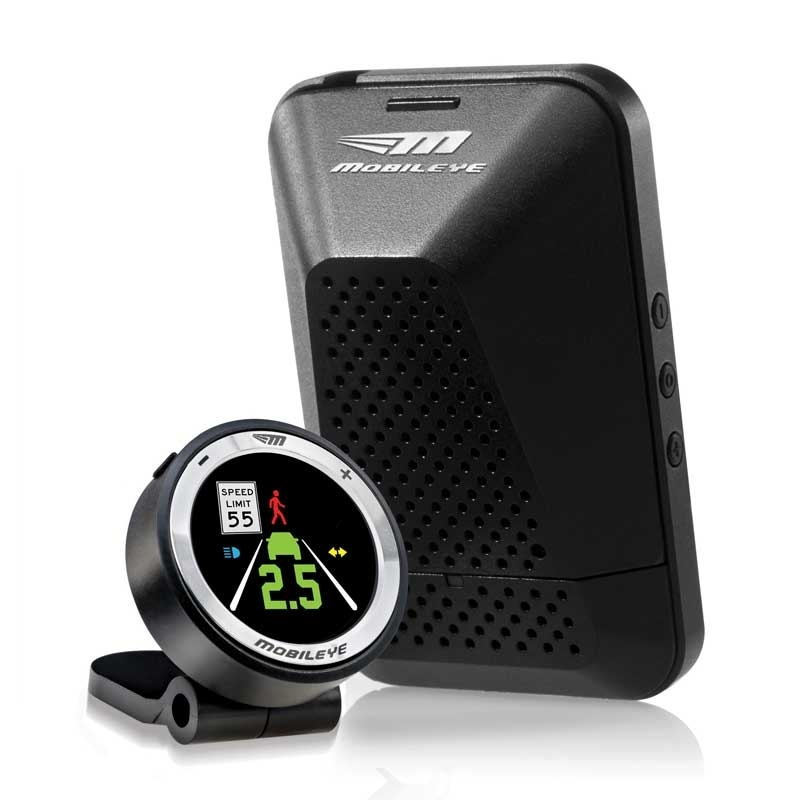
\includegraphics[width=4cm]{figures/4.1.jpg}
    \caption{Mobileye. Fuente: gofleet.com}
    \label{fig:4.1}
\end{minipage}
\begin{minipage}{.5\textwidth} 
\setlength{\parskip}{0.2cm}
\textbf{CARACTERÍSTICAS MOBILEYE}
\begin{itemize}
    \item Frecuencia de detección: 10 Hz
    \item Distancia de alcance: 150 metros
    \item Ángulo de visión horizontal: 74º
    \item Reconocimiento de señales
    \item Reconocimiento del tipo de vehículo
    \item Reconocimiento del estatus del vehículo
\end{itemize}
\end{minipage}
\end{figure}

Por otro lado, la tecnología \gls{lidar} se basa en un láser rotativo para detección de objetos y posterior transformación en una nube de puntos. Los haces de luz proyectan sobre los elementos del entorno, devolviendo a su regreso las variables de posición en el espacio y de intensidad, la cual es dependiente de la reflectividad de cada cuerpo y muy útil para la identificación de diferentes materiales.

El \gls{lidar} utilizado consta de 64 haces o capas, del fabricante Ouster versión OS1 (Figura \ref{fig:4.2}), y se ubica en el techo del vehículo mediante una fijación mecánica. A continuación, se detallan las características del Ouster OS-1.

\newpage
\begin{figure}[htb]
\centering
\begin{minipage}{.4\textwidth}
    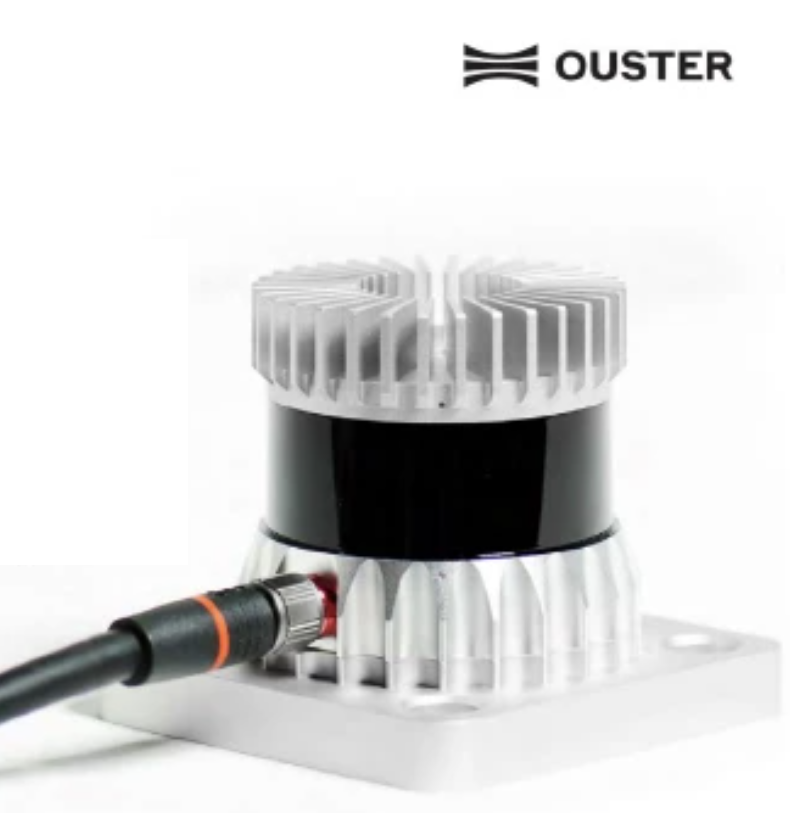
\includegraphics[width=4cm]{figures/4.2.png}
    \caption{Ouster OS1. Fuerte: Ouster/General Laser}
    \label{fig:4.2}
\end{minipage}
\begin{minipage}{.5\textwidth} 
\setlength{\parskip}{0.2cm}
\textbf{CARACTERÍSTICAS OUSTER OS-1}
\begin{itemize}
    \item Frecuencia de rotación: 10 Hz o 20 Hz
    \item Distancia de alcance: 120 metros
    \item Resolución horizontal: 512, 1024 o 2048
    \item Ángulo de visión: 45º (±22.5º)
    \item Resolución angular vertical: 0.35º - 2.8º
    \item Precisión: ±0.7 – 5 centímetros
    \item Puntos por segundo: 1310720
\end{itemize}
\end{minipage}
\end{figure}

Los datos obtenidos del \gls{lidar} se expresan en forma de nube de puntos que se registran por cada frame que captura. Para el correcto análisis de los puntos, es preciso utilizar un algoritmo de clusterización o agrupamiento que nos permita conocer el centro geométrico de cada obstáculo en el espacio. Los algoritmos de clusterización tienen como objetivo formar subgrupos o clusters sobre un conjunto de datos según criterio. Para ello se ha hecho uso del algoritmo planteado en \textcite{clavijo} basado en el método DBSCAN (\gls{dbscan}) adaptado a láseres rotativos, en el que se propone implementar una densidad de puntos variable en función de la distancia al origen. Esta modificación permite aumentar la identificación de clusters de 10 a 40 metros (Figura \ref{fig:4.3}), lo cual favorece directamente a la detección de obstáculos en los ensayos de conducción en vías de alta capacidad propuestos en esta Tesis.

\begin{figure}[h]
    \centering
    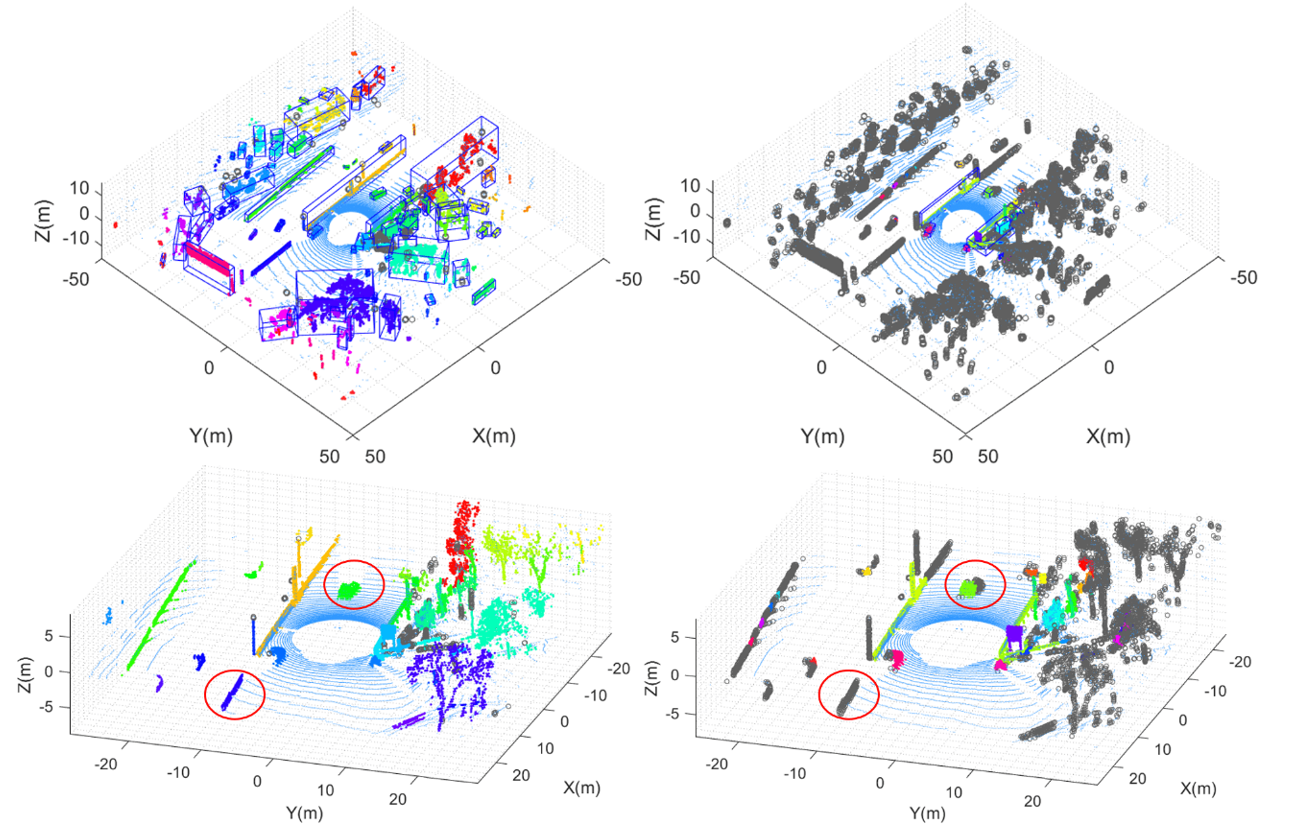
\includegraphics[width=12.5cm]
    {figures/4.3.png}
    \caption{ \label{fig:4.3} Mejora en el funcionamiento del algoritmo de detección en láseres rotativos (\cite{clavijo})}
\end{figure}

El análisis de la mirada se realizó utilizando el sistema de seguimiento visual Tobii Pro Glasses 2 descrito en el subapartado \hyperref[3121]{3.1.2.1.}

Por último, para conocer el movimiento de la cabeza, se elaboró un sistema basado en infrarrojos. El emisor se compuso de tres indicadores lumínicos (Figura \ref{fig:4.4}) montados sobre una gorra junto al circuito integrado y la batería, la cual llevaría el conductor durante los ensayos (Figura \ref{fig:4.6}) basándonos en el sistema de TrackHat. Para el receptor se utilizó una pequeña cámara HD tipo webcam (Figura \ref{fig:4.5}) fácilmente instalable en cualquier parte del vehículo, a la cual se le incorporó un filtro infrarrojo proveniente del Wiimote (Figura \ref{fig:4.7}) que opera en longitudes de onda superiores a 850nm. Las especificaciones de los componentes se adjuntan a continuación.

\begin{figure}[htb]
\centering
\begin{minipage}{.4\textwidth}
    \centering
    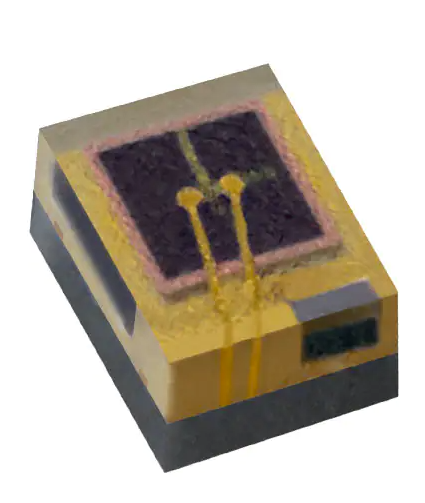
\includegraphics[width=3cm]{figures/4.4.png}
    \caption{LED IR de montaje superficial}
    \label{fig:4.4}
\end{minipage}
\begin{minipage}{.5\textwidth} 
\setlength{\parskip}{0.2cm}
\textbf{CARACTERÍSTICAS LED IR}
\begin{itemize}
    \item Longitud de Onda de Pico: 940 nm
    \item Flujo Radiante: 1.150mW
    \item Intensidad Radiante: 300mW/sr
    \item Tipo de Montaje: Superficial
    \item Ángulo de Intensidad Media: 150º
    \item Tensión de Alimentación Máxima: 3.4V
\end{itemize}
\end{minipage}
\end{figure}

\begin{figure}[htb]
\centering
\begin{minipage}{.4\textwidth}
    \centering
    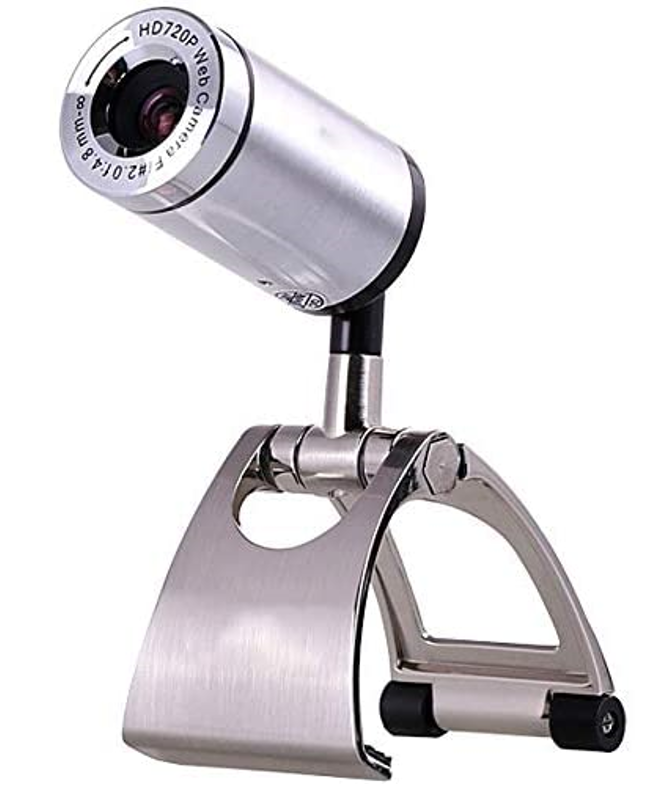
\includegraphics[width=3cm]{figures/4.5.png}
    \caption{WebCam}
    \label{fig:4.5}
\end{minipage}
\begin{minipage}{.5\textwidth} 
\setlength{\parskip}{0.2cm}
\textbf{CARACTERÍSTICAS WEBCAM}
\begin{itemize}
    \item Resolución de Video: 1280 x 720
    \item Modo de Video: YUY2/MJPG
    \item Iluminación Mínima: 10lux
    \item Frames por Segundo: 30fps
    \item Conexión: USB2.0/USB1.1
    \item Alimentación: 5V
\end{itemize}
\end{minipage}
\end{figure}

\begin{figure}[h]
  \centering
  \begin{subfigure}[b]{0.40\textwidth}
    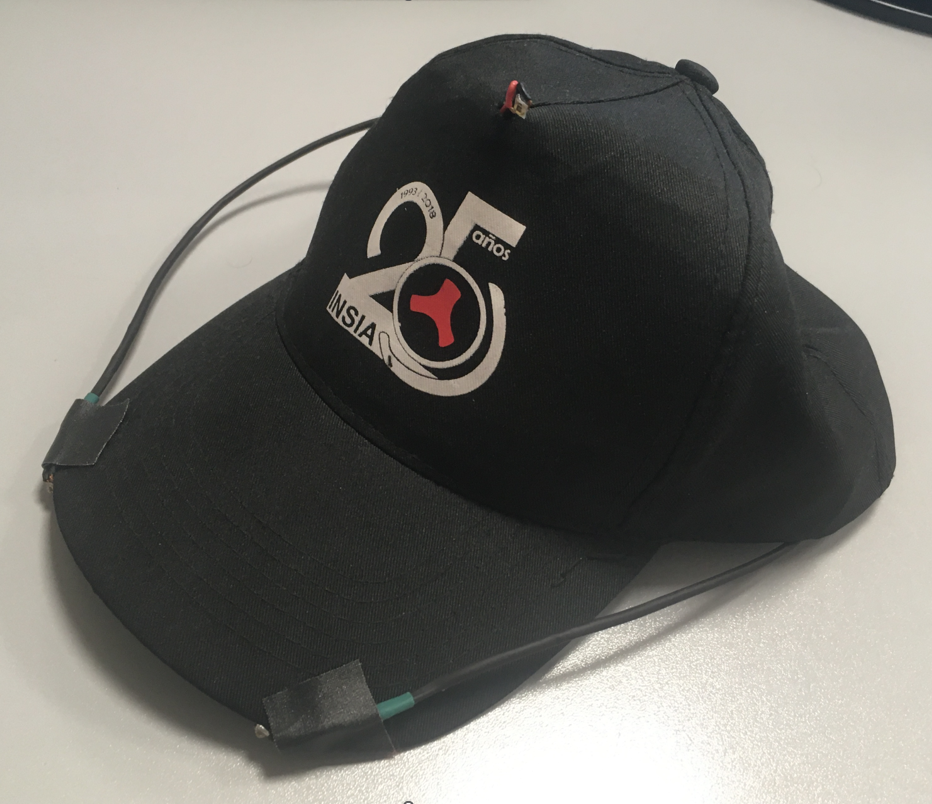
\includegraphics[width=5.5cm]{figures/4.6a.png}
    \caption{}
    \label{fig:4.6a}
  \end{subfigure}
  \hfill
  \begin{subfigure}[b]{0.4\textwidth}
    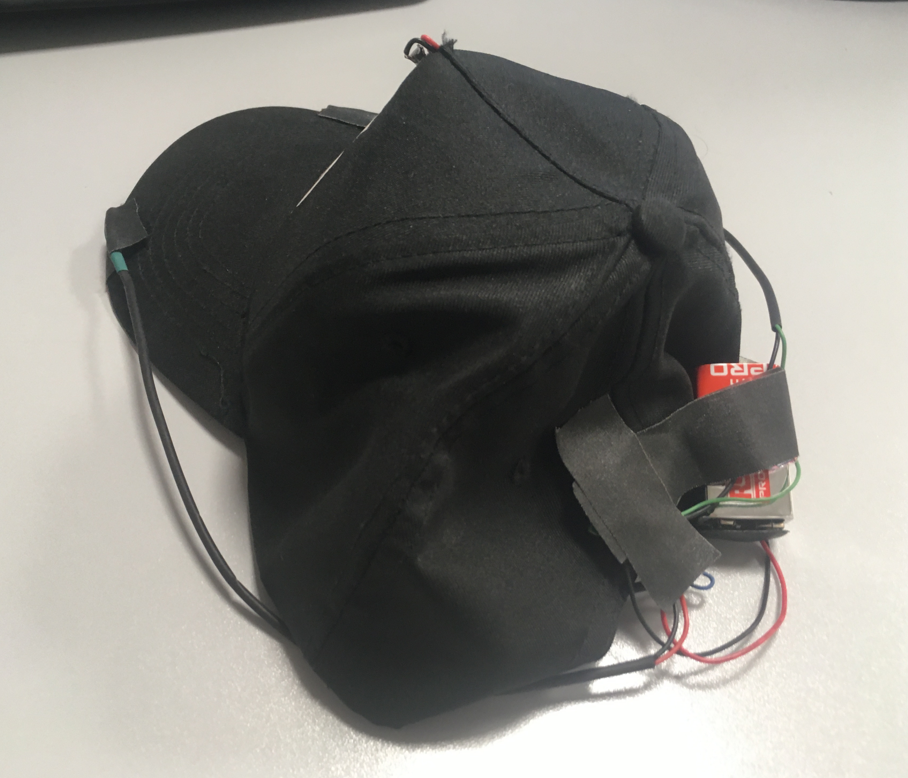
\includegraphics[width=5.5cm]{figures/4.6b.png}
    \caption{}
    \label{fig:4.6b}
  \end{subfigure}
  \caption{Montaje de los infrarrojos sobre gorra. (a) Vista frontal. (b) Vista trasera}
  \label{fig:4.6}
\end{figure}

\begin{figure}[h]
    \centering
    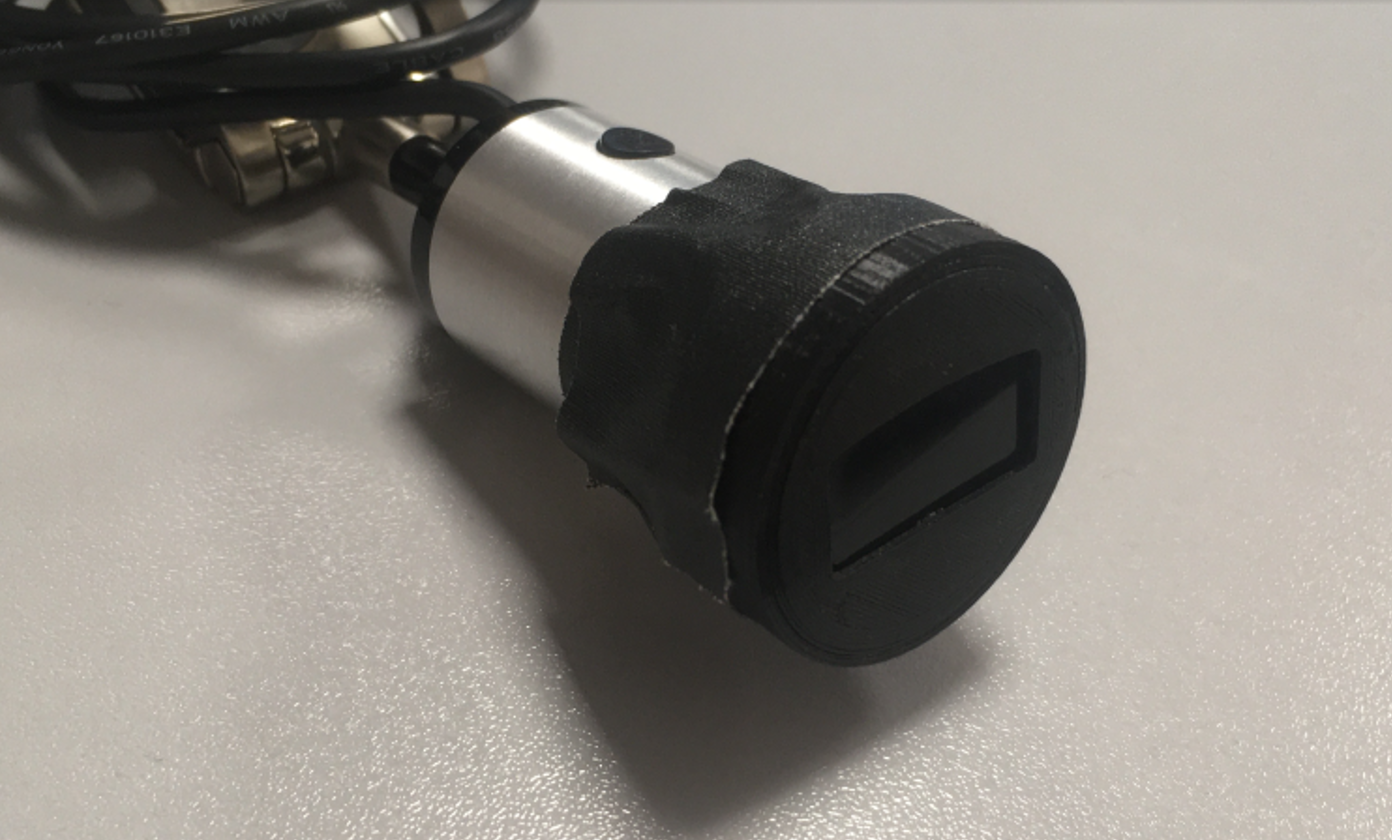
\includegraphics[width=10cm]
    {figures/4.7.png}
    \caption{ \label{fig:4.7} Cámara Webcam}
\end{figure}

La instalación de la cámara se realiza en el salpicadero del vehículo (Figura \ref{fig:4.8}), pudiendo detectar la cabeza del conductor en un amplio rango de movimientos al igual que los sistemas basados en reconocimiento facial, con la ventaja de solo disponer de una única cámara debido al sistema de infrarrojos. 

\begin{figure}[hb]
    \centering
    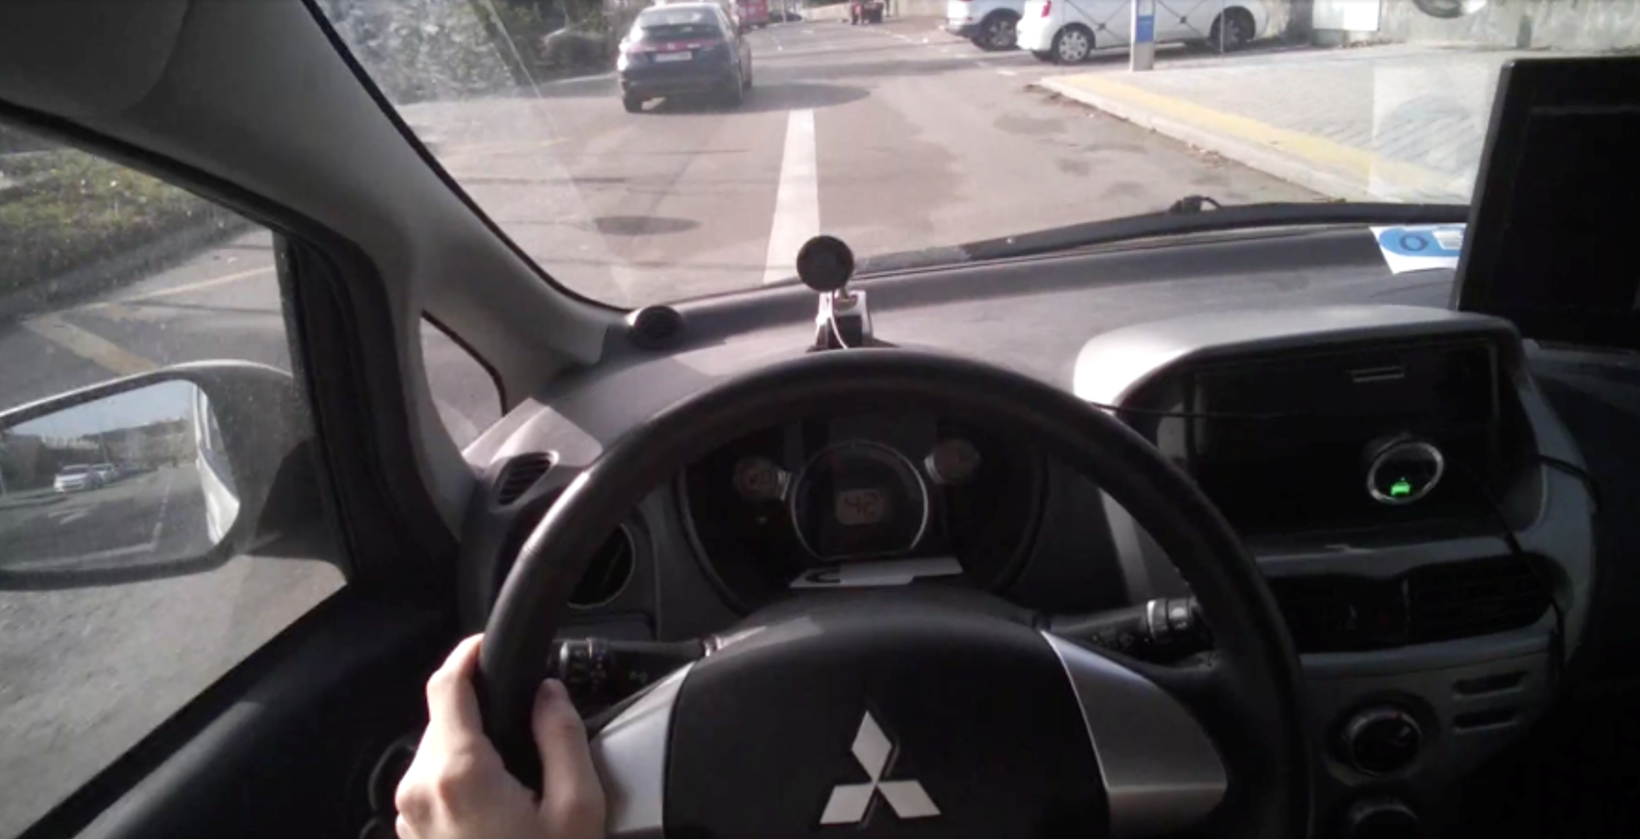
\includegraphics[width=11cm]
    {figures/4.8.png}
    \caption{ \label{fig:4.8} Montaje de la cámara en el interior del vehículo}
\end{figure}

Para la detección de los tres indicadores infrarrojos se optó por el software de código libre y gratuito Opentrack (\cite{opentrack}), comúnmente utilizado en el sector de los videojuegos destacando por su estabilidad y su interfaz configurable frente a otros softwares de pago. El programa realiza una triangulación de dimensiones fijas de los tres indicadores lumínicos detectados y calcula los ángulos de guiñada, alabeo y cabeceo, además de la traslación en los ejes XYZ. Previamente, se realiza una breve configuración donde se especifica que la distribución de los infrarrojos será encima de una gorra y las distancias entre los mismos. Además de trabajar en tiempo real, Opentrack es capaz de exportar los datos de la grabación para poder trabajar con ellos a posteriori. Los datos se muestran tanto en bruto como tras un filtro y un suavizado personalizables, que favorecen la linealidad de los resultados y eliminan ruido y valores pico de la adquisición. Para los ensayos se ha utilizado el Filtro \emph{“Accela”}, con valores de 0.03º para zona muerta y de 1.5º de suavizado para rotación, y de 0.1 milímetros de zona muerta y 1 milímetro de suavizado para traslación. A su vez, se realizan ajustes en los ejes de coordenadas para una buena compenetración con los datos obtenidos del sistema de seguimiento visual. 

Todos los sensores son referenciados y ubicados en un vehículo instrumentado, concretamente el Mitsubishi iMiEV que se puede observar en la figura \ref{fig:4.9}.

\begin{figure}[h]
    \centering
    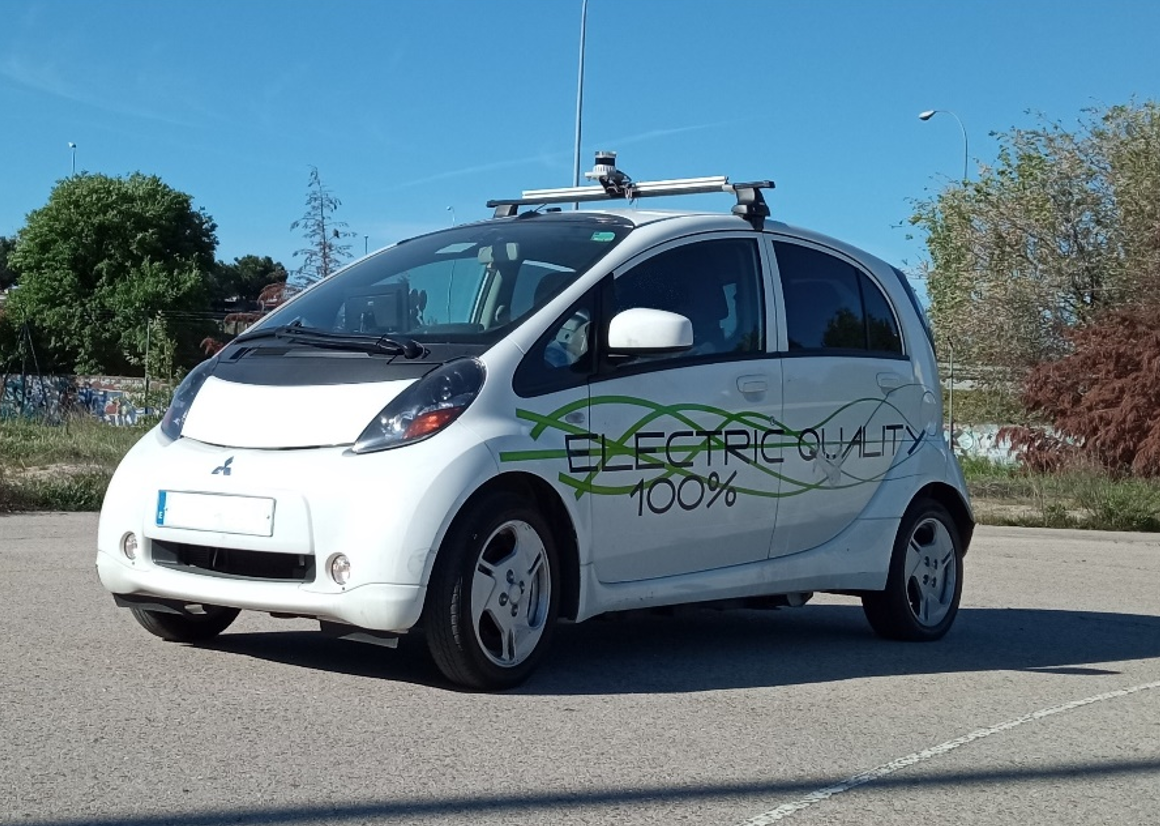
\includegraphics[width=9cm]
    {figures/4.9.png}
    \caption{ \label{fig:4.9} Vehículo Mitsubishi iMiEV instrumentado}
\end{figure}

Los sistemas se conectan a un ordenador encargado del bajo nivel, basado en el sistema operativo GNU/Linux con el entorno de trabajo ROS (Robotic Operating System). La creación de un reloj temporal común a todos los sistemas y la adquisición a la misma frecuencia han sido las principales razones para la elección de este entorno de desarrollo.
Además de los sistemas mencionados anteriormente, se recogerán datos del BUSCAN, para conocer las variables del vehículo, y de un receptor \gls{gps} Trimble R4, instalado en el vehículo para mejorar conocer el posicionamiento del vehículo en los ensayos.

\section{Ajuste y comprobación del sistema de percepción del conductor }\label{43}

Previo al análisis de correlación de la mirada del conductor en el espacio, se realizaron una serie comprobaciones y ajustes de los sistemas de percepción del conductor expuestos en este capítulo, donde se evalúa la integración del sistema de seguimiento de la cabeza junto a los datos de seguimiento visual, calculando la precisión o repetibilidad, y la exactitud resultante en el sistema de coordenadas global.

\subsection{Proyección de la mirada en el sistema de coordenadas global}\label{431}

El sistema de seguimiento visual empleado proporciona la capacidad de exportar numerosas variables en diversos formatos, en concreto la dirección de la dirección de la mirada en el sistema de coordenadas global en 2D, en los ejes XY, y en 3D, en los ejes XYZ. A pesar de que la mirada en 2D está en formato pixeles y la mirada en 3D en metros, una superposición de los datos en el plano XY debería proporcionar una imagen similar en ambos formatos. Sin embargo, al observar diferencias entre ambos formatos, se procedió a analizar la adquisición del sistema con el fin de asegurar una fuente de datos óptima.

Para evaluar la correlación entre las variables de la mirada en 2D y 3D se propone el siguiente ensayo, replicando el procedimiento que el fabricante realizó para la determinación de la exactitud y precisión, o repetibilidad (\cite{tobii}). Los participantes deben de mirar a 4 dianas en forma de cruz ubicadas en una pared estática con una quinta diana de referencia en el centro. Dado que las gafas disponen de una resolución de 1920 x 1080 píxeles, se procede a calcular la distancia necesaria para la realización del ensayo, asegurando que la imagen capturada por la cámara tenga las mismas medidas en milímetros que en píxeles. Esta distancia es de 1.1 metros, encontrándose además dentro del rango óptimo de valores que defiende el fabricante para la obtención de buenos resultados (máximo 3 metros de distancia al objetivo observado (\cite{tobii}). Los ángulos que forman las dianas con la horizontal son 5º, 10º, 15º y 20º, tal y como se muestra en la figura \ref{fig:4.10}, y se restringe el movimiento de la cabeza para analizar puramente la dirección de la mirada.

\begin{figure}[h]
    \centering
    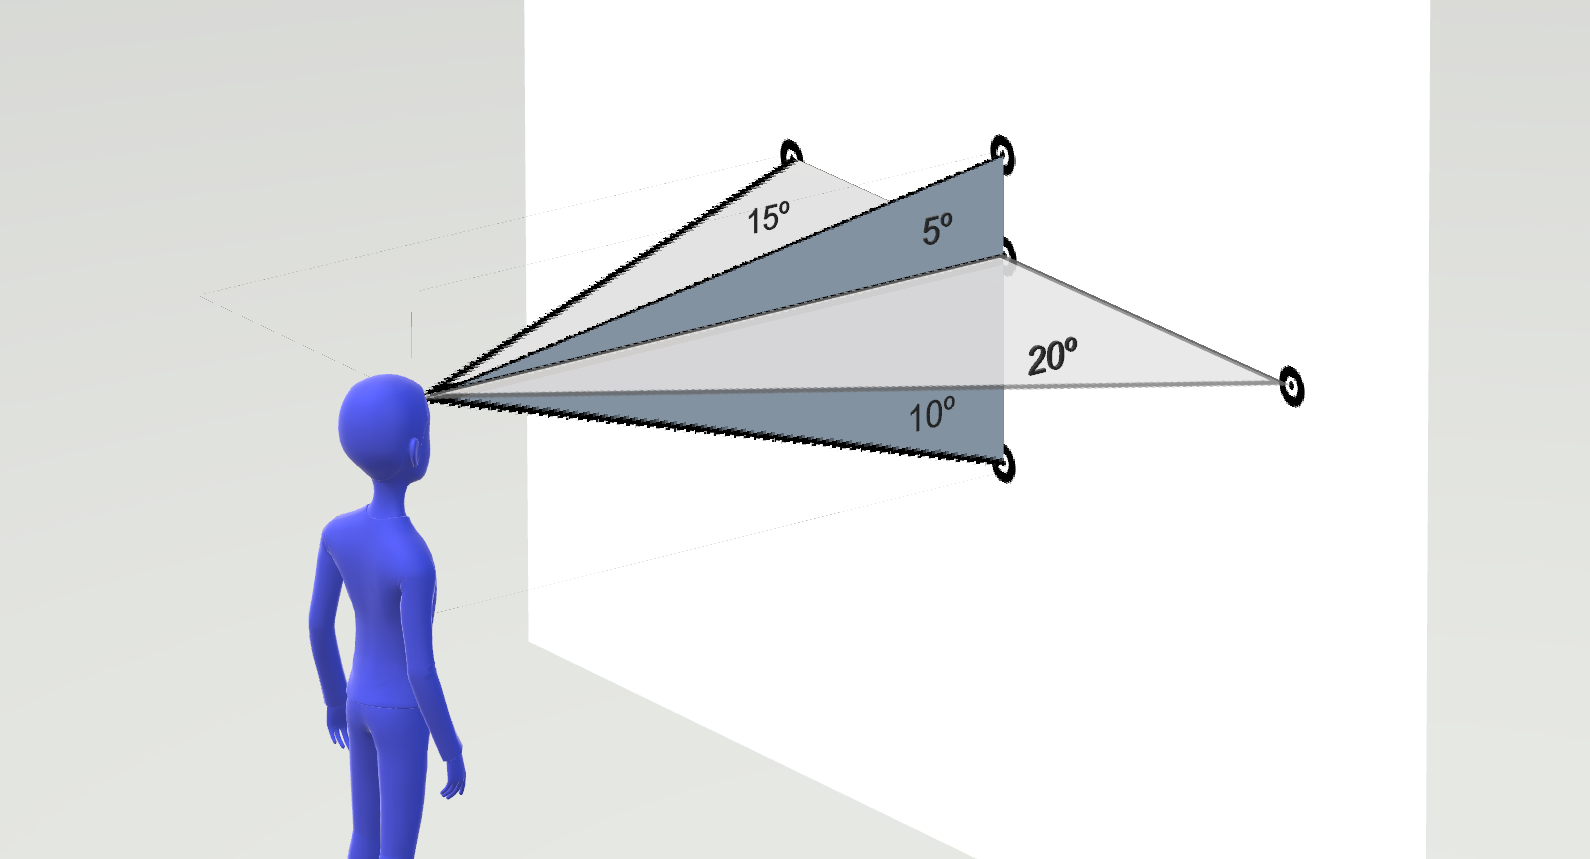
\includegraphics[width=9cm]
    {figures/4.10.png}
    \caption{ \label{fig:4.10} Posicionamiento de las dianas para integración del sistema de percepción del conductor}
\end{figure}

En la siguiente imagen (Figura \ref{fig:4.11}) se observa que existen diferencias notables entre las dos variables, aun perteneciendo ambas al mismo ensayo, correspondiente al sujeto piloto.

\vspace{-10pt}
\begin{figure}[h]
    \centering
    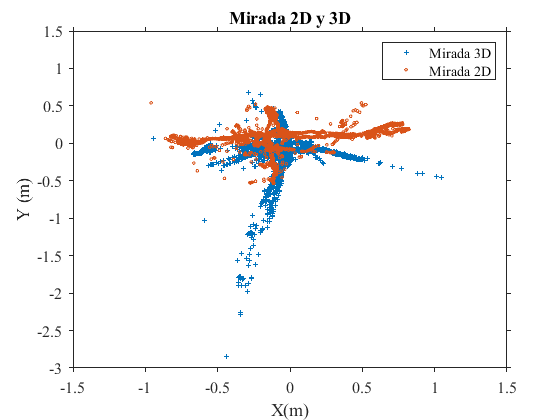
\includegraphics[width=10cm]
    {figures/4.11.png}
    \caption{ \label{fig:4.11} Posición de la mirada en 2D y 3D en ensayo piloto}
\end{figure}

La razón por la que se produce este fenómeno fue revelada analizando la posición de la variable en el eje Z (profundidad en este caso). Se observa que el haz que proyecta la mirada del conductor hacia un objeto detectaba dicho punto mucho más lejos de lo que realmente esta, viéndose también distorsionadas por trigonometría las distancias en los ejes X e Y.
En la figura \ref{fig:4.12} se puede observar el valor de la distancia en el eje Z para el ensayo anterior, donde se muestra que los datos son erráticos e inestables en ciertos puntos, estando la línea de tendencia de la gráfica a 0.841 metros, valor próximo a los 1.1 metros a los que se realiza el ensayo.

\vspace{-15pt}
\begin{figure}[h]
    \centering
    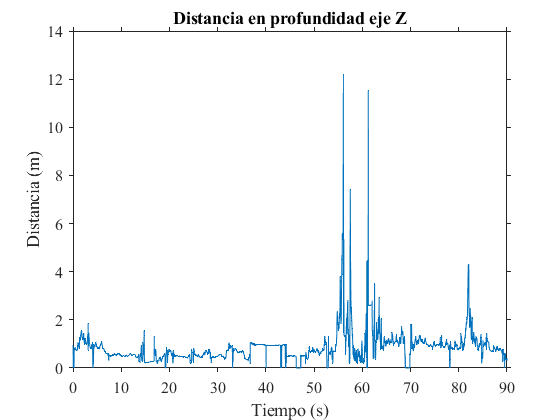
\includegraphics[width=9cm]
    {figures/4.12.png}
    \caption{ \label{fig:4.12} Distancia en profundidad eje Z en ensayo piloto}
\end{figure}

Para solventar este problema, se propone forzar la variable de profundidad en el eje Z a la distancia fija de 1.1 metros a la que se realizó el ensayo anterior, dado que los puntos en este eje no pueden ser superiores a este valor, y se calcula por trigonometría los valores del haz en los ejes X e Y. Los resultados se ven reflejados en la figura \ref{fig:4.13}, donde la posición de la mirada en 3D ha sido corregida, observándose un patrón similar al registrado por las variables en 2D.

\vspace{-15pt}
\begin{figure}[h]
    \centering
    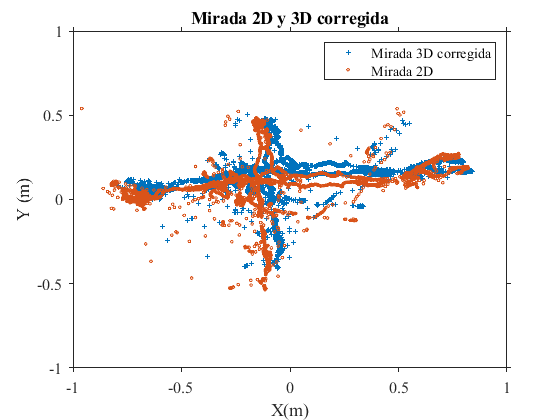
\includegraphics[width=10cm]
    {figures/4.13.png}
    \caption{ \label{fig:4.13} Posición de la mirada en 2D y 3D corregida}
\end{figure}

\newpage
\subsection{Integración del sistema de movimiento de la cabeza }\label{432}

El sistema de coordenadas global de los ensayos propuestos en la presente Tesis tiene su cero en la base de la cabeza del conductor, donde se producen los giros en los tres ejes. El sistema de seguimiento de la cabeza genera variables de los ángulos de rotación y de la translación en XYZ. Estas variables realizan la corrección de los datos de la mirada que se resuelve mediante un sistema matricial, donde, por una parte, se transforman los ángulos con la matriz de rotación de Euler (Eq. \ref{eq:4}), y posteriormente se aplica una matriz de traslación (Eq. \ref{eq:5}). Los datos del sistema de seguimiento visual (Eq. \ref{eq:6}) son multiplicados matricialmente por la matriz de transformación compuesta por la rotación y la translación como se observa en la ecuación \ref{eq:7}.


\begin{equation}\label{eq:4}
\text{Euler} = \begin{bmatrix}
\alpha_x & \beta_x & \gamma_x \\
\alpha_y & \beta_y & \gamma_y \\
\alpha_z & \beta_z & \gamma_z
\end{bmatrix}
\end{equation}

\begin{equation}\label{eq:5}
\text{Posición} = \begin{bmatrix}
X_n \\
Y_n \\
Z_n
\end{bmatrix}
\end{equation}

\begin{equation}
\text{Visual} = \begin{bmatrix} \label{eq:6}
x_n \\
y_n \\
z_n \\
1
\end{bmatrix}
\end{equation}

\begin{equation}\label{eq:7}
\text{Correc}_1 = \left[ \text{Euler} | \text{Posición} \right] \cdot \left[ \text{Visual} \right] = \left[ \left[ \begin{array}{@{}c@{}}
\text{Matriz} \\
\text{Rotación} \\ 
\text{Euler} \\
\end{array} \right] \left( \begin{array}{@{}c@{}}
X_n \\
Y_n \\
Z_n \\
\end{array} \right) \right] \cdot \left[ \left( \begin{array}{@{}ccc@{}}
x_n \\
y_n \\
z_n \\
1  \\
\end{array} \right) \right]
\end{equation}

Sabiendo que la incertidumbre de ambos sistemas es alta, pero está dentro de los limites admisibles, se realiza una evaluación meramente cualitativa de la fusión con objeto de comprobar la bondad del sistema desarrollado. Para ello se propone calcular la repetibilidad y la exactitud del ensayo de 4 dianas mencionado anteriormente, para una muestra reducida de 3 sujetos (\emph{N}). La repetibilidad y la exactitud son recursos comúnmente utilizados para la evaluación del error obtenido en sistemas de medición, como se puede apreciar en \textcite{holmqvist}, con la validación de la calidad de los sistemas de seguimiento visual. La exactitud se define como la cercanía de las medidas obtenidas al valor real, mientras que la repetibilidad es el grado de proximidad entre las mediciones. Para la exactitud se toma como referencia la medida real y para la repetibilidad, el centroide de la nube de puntos. Ambas variables indican diferentes aspectos y, por tanto, son independientes, pudiéndose obtener una muestra muy precisa, donde todas las medidas difieren poco entre sí, pero poco exacta si está lejos del valor real.

En la tabla \ref{tab:4.1}, se muestran los resultados obtenidos de la fusión sensorial para el ensayo de las cuatro dianas mencionado anteriormente.

\newpage
\begin{table}[h]
\centering
\begin{tabular}{cccccc}
\multirow{2}{*}{\textbf{Grados (°)}} & \multirow{2}{*}{\textbf{N}} & \multicolumn{2}{c}{\textbf{Exactitud (°)}} & \multicolumn{2}{c}{\textbf{Repetibilidad (°)}} \\ \cline{3-6} 
                                     &                             & \textit{Media}        & \textit{SD}        & \textit{Media}          & \textit{SD}          \\ \hline
5                                    & 3                           & 3.86                  & 3.15               & 3.70                    & 2.44                 \\ \hline
10                                   & 3                           & 2.85                  & 1.33               & 1.06                    & 0.80                 \\ \hline
15                                   & 3                           & 1.51                  & 0.65               & 1.60                    & 0.84                 \\ \hline
20                                   & 3                           & 2.14                  & 0.79               & 0.74                    & 0.52                 \\ \hline
\end{tabular}
\caption{Exactitud y repetibilidad del sistema de percepción del conductor}
\label{tab:4.1}
\end{table}

\vspace{-15pt}
Como era de esperar, la exactitud y la repetibilidad del sistema de seguimiento visual se ven afectadas por la inclusión del sistema de seguimiento de la cabeza. Se observa que los peores resultados se obtienen para el valor de 5°, lo cual puede ser explicado por la proximidad a la diana central y la atracción de la mirada hacia un elemento próximo y similar al objetivo visual. Esta afirmación se refuerza con el valor de dispersión obtenida para esa medida. Otro aspecto a considerar es el número de sujetos, ya que se considera que una mayor población en las muestras adquiridas enriquecería de manera notable los resultados. 

A pesar de las desviaciones detectadas, se puede concluir que la fusión sensorial es más precisa que exacta, donde los datos se agrupan correctamente, pero difieren de la medida real. No obstante, los valores se consideran válidos para la aplicación propuesta, dado que a la distancia máxima operable (50 metros) la desviación supondría 3.3 metros en el peor de los casos, siendo inferior al ancho de un carril de 3.5 metros. 

\section{Análisis de correlación con percepción del entorno}\label{44}
La integración de los sistemas de detección del entorno, la cámara Mobileye y el láser Ouster, ya ha sido estudiada con anterioridad en \textcite{villacieros}, observado ciertas carencias en la redundancia conjunta debido a la naturaleza de los mismos. Por un lado, la versión utilizada para la cámara Mobileye tiene un ángulo de visión horizontal de 74°, por lo que la máxima amplitud de detección para objetos que se sitúan en el lateral del vehículo es de 36°. Además, la localización de obstáculos es menos flexible respecto a la del Ouster, por lo que no permite una buena adaptabilidad a los cambios. Respecto al sensor láser, a pesar de la mejora del algoritmo de clusterización (\cite{clavijo}), es un hecho que, a mayor distancia de detección, mayor distancia entre haces consecutivos, siendo esta una de las principales razones de la pérdida de objetos en el campo visual. 

Debido a las limitaciones presentadas, se propuso en primer lugar, un análisis en la correlación en la detección de obstáculos de la cámara Mobileye y el láser Ouster, y posteriormente, la integración total con el sistema de seguimiento visual.

\subsection{Metodología }\label{441}
Dos vehículos instrumentados realizaron una maniobra de seguimiento de vehículo (car-following) en un entorno abierto, correspondiente a una carretera de urbana. Se realizaron 5 repeticiones del mismo recorrido, detectando al vehículo delantero mediante la cámara Mobileye y el láser Ouster durante todo el ensayo. 

Por otro lado, se registraron datos del conductor a través del sistema de seguimiento visual y se estudió el campo visual del conductor. La visión humana se compone de un campo visual central, correspondiente a la zona de máxima agudeza visual, y un campo visual periférico, situado a los laterales de la zona central y que también aporta información visual al cerebro, pero de manera menos precisa. A menudo, en entornos de conducción, el ángulo de visión central se ve afectado por la velocidad del vehículo, viéndose reducido y repercutiendo directamente en la toma de decisiones. Este fenómeno denominado ``efecto túnel'' y ampliamente estudiado (\cite{edwards}) ha sido integrado en el análisis de correlación para el sistema visual, considerando esta variable como un rango de incertidumbre admisible en la detección de la mirada del conductor.

\subsection{Resultados }\label{442}
El análisis de correlación de los sistemas se calculó en porcentaje de frames de detección frente al número total de frames de la grabación. Primero se calculó la coincidencia entre los sistemas de percepción, cámara y \gls{lidar}, y posteriormente se añadió el sistema de seguimiento visual en el sistema de coordenadas global. 

Un ejemplo de ello se observa en el frame mostrado en la figura \ref{fig:4.14}, donde aparecen todos los sistemas desde la perspectiva de planta, ubicándose el vehículo instrumentado en el punto (0, 0). Los obstáculos detectados por la cámara aparecen con un asterisco rojo, en este caso solo existe el vehículo delantero y el vehículo instrumentado en el centro. Los demás objetos son el resultado de la detección con el láser y el algoritmo de clusterización \gls{dbscan}, mencionado en el apartado \ref{42} instrumentación y procesamiento de datos. En este ejemplo se puede observar que la detección con la cámara coincide con uno de los clusters determinados por la detección del láser. Las líneas verticales representan la dirección de la mirada del conductor, partiendo desde el centro hacia delante, siendo el resultado de la integración del sistema de seguimiento visual y el sistema de movimiento de la cabeza. El triángulo azul muestra el ángulo central de visión del conductor, el cual pivota según la dirección de la mirada y cambia su apertura en función de la velocidad del vehículo, englobando la dispersión de miradas admisibles.

Como se observa en la figura \ref{fig:4.14}, dentro de este ángulo se encuentra la dirección de la mirada y el vehículo delantero.

\vspace{-20pt}
\begin{figure}[h]
    \centering
    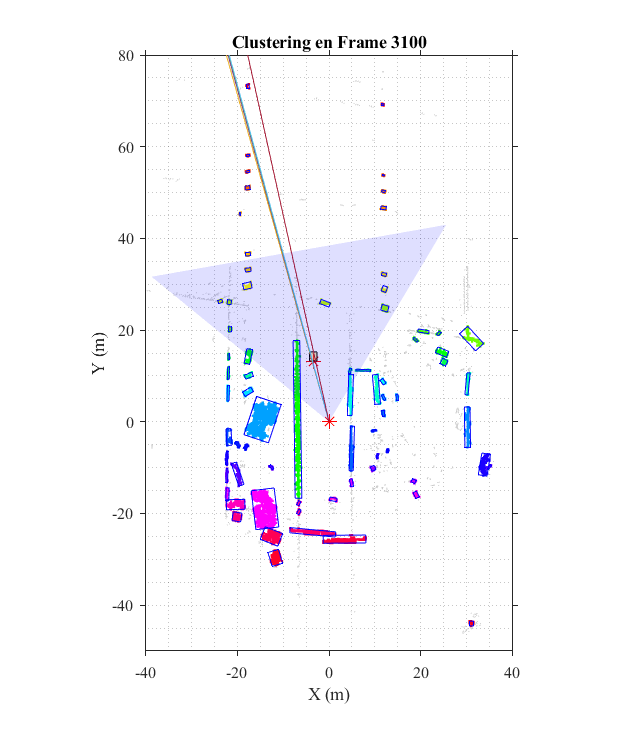
\includegraphics[width=9.5cm]
    {figures/4.14.png}
    \caption{ \label{fig:4.14} Mirada del conductor a un obstáculo mediante la fusión de todos los sistemas}
\end{figure}

\newpage
Los porcentajes de detección de frames para la cámara Mobileye, el láser Ouster y la detección conjunta, se muestran en la siguiente tabla \ref{tab:4.2}, donde los resultados de la detección conjunta son relativamente bajos y destaca positivamente la detección realizada por la cámara Mobileye.

\begin{table}[h]
\centering
\begin{tabular}{cccccc}
\textbf{Ensayo}       & \textbf{1}   & \textbf{2}     & \textbf{3}     & \textbf{4}     & \textbf{5}     \\ \hline
\% detección Mobileye & 100 & 87.31 & 73.05 & 92.43 & 95.18 \\ \hline
\% detección Ouster   & 81.36        & 74.02          & 65.25          & 58.37          & 100            \\ \hline
\% detección conjunta & 81.36        & 61.93          & 39.01          & 50.81          & 95.18         
\end{tabular}
\caption{Porcentaje de correlación en frames de Mobileye y Ouster}
\label{tab:4.2}
\end{table}

De igual manera, los resultados se muestran en porcentajes de frames detectados respecto al total de frames, mostrando por un lado la coincidencia de miradas al obstáculo detectado, y por otro, la coincidencia de miradas dentro del ángulo de visión central en función de la velocidad y el giro de la cabeza (Tabla \ref{tab:4.3}). Los haces de la mirada se han distribuido en grupos de cinco, debido a que el registro de la actividad ocular funciona a 50 Hz, cinco veces superior al resto de los sistemas, considerándose suficiente muestreo para este análisis. 

\begin{table}[h]
\centering
\begin{tabular}{cccccc}
\textbf{Ensayo}                                          & \textbf{1} & \textbf{2} & \textbf{3} & \textbf{4} & \textbf{5} \\ \hline
\% coincidencia de miradas al   obstáculo                & 13.66      & 38.67      & 58.86      & 32.97      & 39.01      \\ \hline
\% coincidencia de miradas en   ángulo de visión central & 59.62      & 93.95      & 99.29      & 96.21      & 88.83      \\ \hline
\end{tabular}
\caption{Porcentaje de correlación en \\ frames del sistema de seguimiento visual}
\label{tab:4.3}
\end{table}

Los valores obtenidos indican que el conductor realiza la mayor parte de las miradas dentro del ángulo de visión central y, como mínimo un 30\% de las miradas al obstáculo en concreto, exceptuando el ensayo 1 en ambos casos. Los valores más bajos se debieron a diversos problemas en la adquisición de la mirada, como es el caso del ensayo 1, donde se dieron situaciones en las que el conductor giraba en exceso la cabeza, perdiendo una de las señales de triangulación del sistema de seguimiento y proyectando los haces de la mirada de manera incorrecta. A pesar de que se eligieron sensores infrarrojos por su buena adaptabilidad a las diferencias lumínicas, el exceso de luz en ciertas zonas junto a destellos puntuales también afectó a la descalibración del sistema, traduciéndose en una pérdida parcial de los datos.

\subsection{Discusión}\label{443}
La detección de obstáculos es una función crítica para la seguridad en el manejo de vehículos. En este estudio se realizaron ensayos de detección en conducción real fusionando dos sistemas de percepción del entorno y un sistema de seguimiento visual, referenciado al sistema de coordenadas global a través de un sistema de seguimiento de la cabeza.

En los resultados obtenidos sobre el análisis de correlación se encontró que la detección para la cámara Mobileye fue alta, pero que debido a la baja detección del \gls{lidar} Ouster relacionada con la clusterización de obstáculos a largas distancias, la efectividad conjunta se vio mermada de manera general. Con respecto al análisis de la fusión junto al sistema de seguimiento visual, se presupone que el conductor dedicará gran parte de su atención al vehículo que circula delante de él. Sin embargo, esta hipótesis no es del todo cierta ya es posible adquirir información de la escena sin necesidad de mirar directamente al obstáculo que se encuentra en frente, como se puede ver en los resultados obtenidos de miradas en el ángulo de visión central calculado a través del “efecto túnel”. Los resultados obtenidos mostraron que un gran porcentaje de las miradas coincidieron con el ángulo de visión central pero solo un tercio de las mismas alcanzaron al vehículo delantero. 

\section{Conclusiones}\label{45}
La conducción autónoma se basa principalmente en la adquisición de información del entorno a través de diferentes sensores, la cual se procesa como lo haría un conductor humano. La redundancia entre sensores ofrece una mejora en los algoritmos de control, haciendo que la integración de los vehículos en el tráfico mixto sea lo más eficaz posible. Dado que todavía queda mucho conocimiento sobre la conducción humana que implementar, se considera que la proyección de la mirada del conductor hacia el entorno exterior puede aportar una valiosa información en la determinación de reglas del sistema de decisiones.

En este capítulo se ha realizado una fusión sensorial entre dos sistemas de detección de obstáculos y un sistema de seguimiento visual referenciado al sistema de coordenadas global gracias a un sistema para el seguimiento de la cabeza. Este desarrollo ha permitido obtener un conocimiento global de la mirada del conductor hacia el entorno exterior, facilitando su integración con otros sistemas de percepción del entorno. No obstante, el sistema de seguimiento de la cabeza no se considera robusto dado que los resultados muestran problemas en la adquisición de datos debido a sus carencias frente a las variaciones lumínicas y la movilidad del conductor. En futuros estudios se considera interesante la implementación de dos cámaras que capturen dicho movimiento y aporten redundancia a la adquisición.

En los ensayos realizados en conducción real, los sensores de percepción del entorno han tenido buenos resultados en la detección individual, pero mejorables en la detección conjunta, debido a las limitaciones del método de clusterización para el entorno ensayado. Tras la adición del sistema de seguimiento visual referenciado al sistema global se observó que, en la mayoría de los ensayos, la mirada del conductor se encontraba dentro del ángulo central de visión, pero que solo una tercera parte de las mismas se realizaban al obstáculo en concreto. Este hecho refuerza la hipótesis de que el conductor puede recopilar información de la escena sin requerir una visión precisa, recalcando la importancia de la visión periférica.

En el siguiente capítulo se recogerán datos de conducción real, haciendo uso de los desarrollos de fusión obtenidos, para el desarrollo de un modelo de conducción enfocado a la conducción autónoma. 
